\Chapter{REVUE DE LITTÉRATURE}\label{sec:RevLitt}

%%%% -------------- %%%%
\section{Title of section}

\lipsum[2-4]

%%%% -------------- %%%%
\subsection{Title of subsection}
\subsubsection{Title of subsubsection}

$g_{moon}$=\SI{1.62}{\meter\per\square\second}

\SI{120}{\degreeCelsius} 

%-178°C 

\cite{williams2017global}

% \citeA{williams2017global}


See the table \ref{tab:lauch_environment} 

\begin{table}%[h]  %Do not use [h] or [H], let LaTeX place the figure
    \centering
    \begin{tabular}{|>{\columncolor[gray]{0.93}}c|c|L|L|c|}\hline
    \rowcolor[gray]{0.93}\diagbox{\textbf{Source}}{\textbf{Charge}} & Acoustique & Vibration aléatoire & Vibration sinusoïdale & Choc \\ \hline
    Décolage              & X & X &   &   \\ \hline
    Aérodynamique         & X & X &   &   \\ \hline
    Phases de séparation  &   &   &   & X \\ \hline
    Combustion du moteur  &   & X & X &   \\ \hline
    \end{tabular}
    \caption{Sources de charge stochastique pendant un lancement de fusée \cite{yunis2005standard}}
    \label{tab:lauch_environment}
\end{table}

Full figure : \ref{fig:Falcon9} 
Sub figure : \ref{fig:falcon9_static} 

\begin{figure}%[H] %Do not use [h] or [H], let LaTeX place the figure
     \centering
     \begin{subfigure}[]{0.48\textwidth}
         \centering
         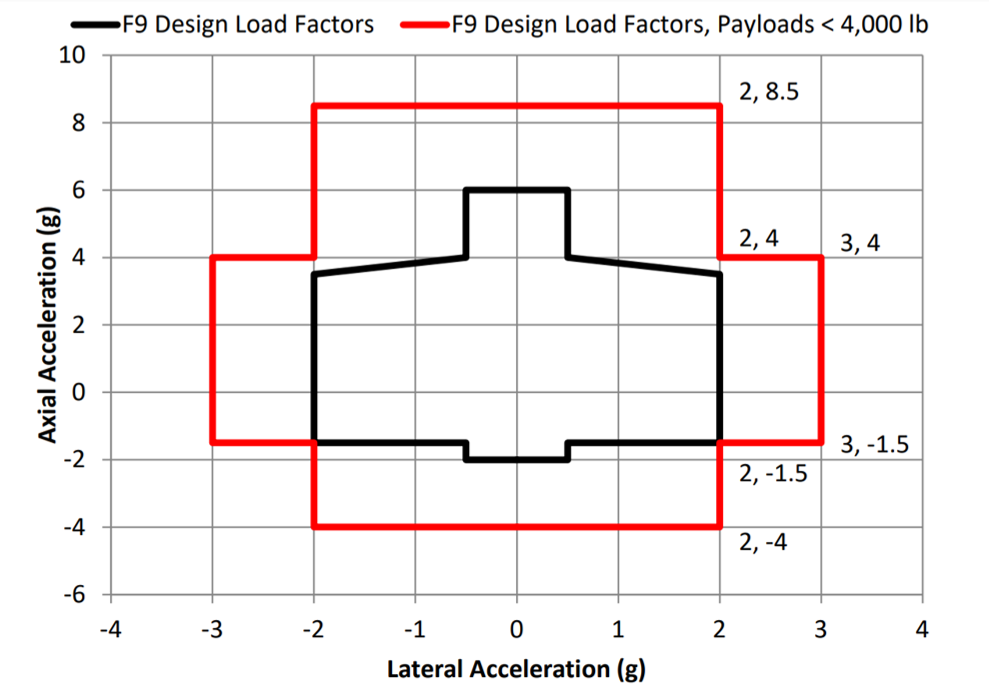
\includegraphics[width=\textwidth]{Img/falcon_static.png}
         \caption{Accélérations statiques axiales et latérales maximales}
         \label{fig:falcon9_static}
     \end{subfigure}
     \hfill
     \begin{subfigure}[]{0.48\textwidth}
         \centering
         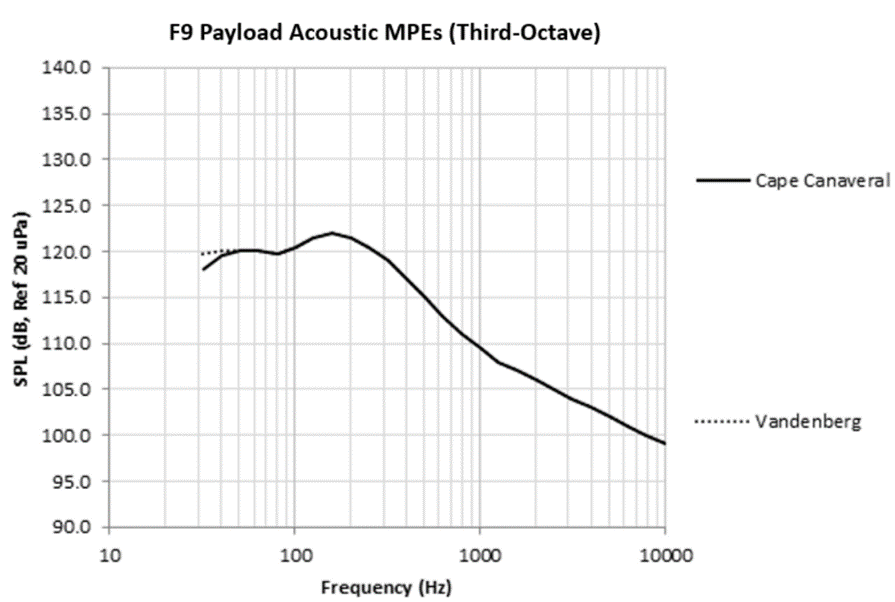
\includegraphics[width=\textwidth]{Img/falcon_acoustic.png}
         \caption{Environnement acoustique maximal prédit (P95/50)}
         \label{fig:falcon9_acoustic}
     \end{subfigure}
     \\
     \begin{subfigure}[]{0.48\textwidth}
         \centering
         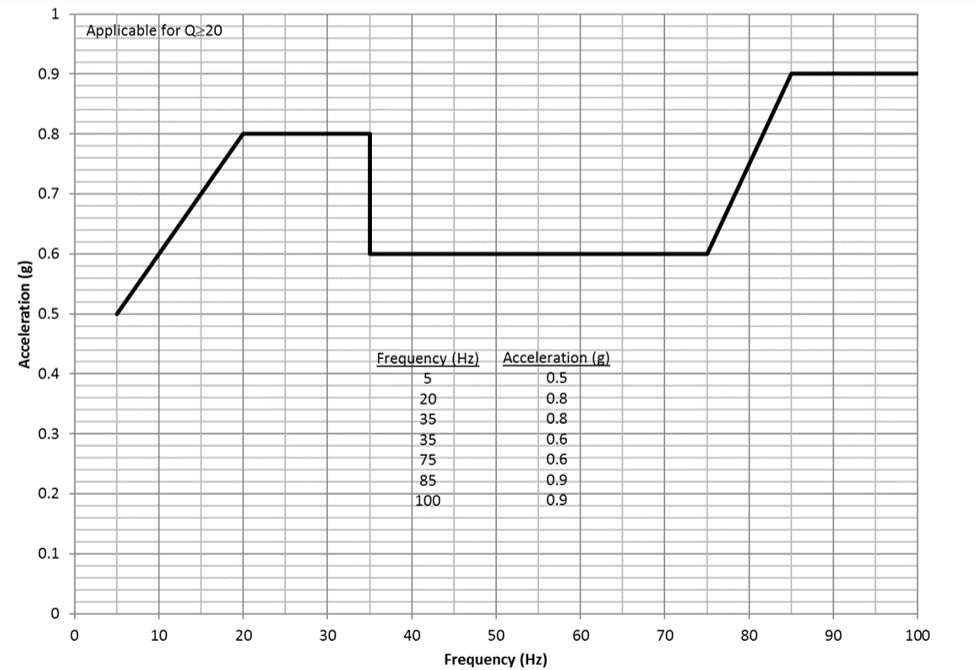
\includegraphics[width=\textwidth]{Img/falcon_sine.png}
         \caption{Environnement de vibration sinusoïdal maximal équivalent}
         \label{fig:falcon_sine}
     \end{subfigure}
     \hfill     
     \begin{subfigure}[]{0.48\textwidth}
         \centering
         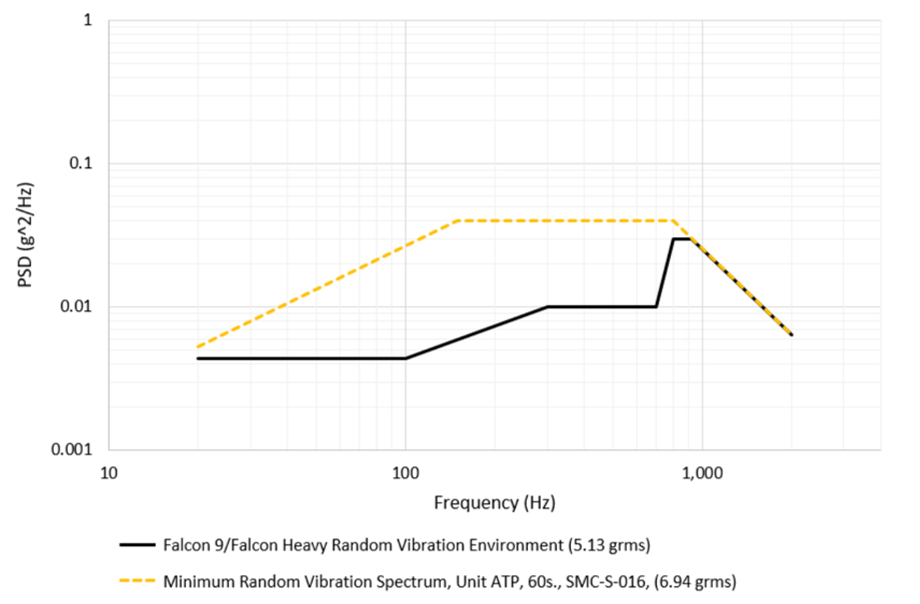
\includegraphics[width=\textwidth]{Img/falcon_random.png}
         \caption{Environnement de vibrations aléatoires maximum prédit (P95/50)}
         \label{fig:falcon_random}
     \end{subfigure}
     \caption{\centering{Charges maximales exercées sur le rover par l'environnement du lancement de la fusée Falcon 9. Tiré de \cite{SpaceExplorationTechnologiesCorp2020FalconGuide} } }.
     \label{fig:Falcon9}
\end{figure}



\begin{equation}
\begin{bmatrix}
\varepsilon_{11} \\
\varepsilon_{22} \\
\gamma_{12} \\
\end{bmatrix}
=
\begin{bmatrix}
1/E_{11} & -\nu_{12}/E_{11} & 0 \\
-\nu_{12}/E_{11} & 1/E_{22} & 0 \\
0 & 0 & 1/G_{12} \\
\end{bmatrix}
\begin{bmatrix}
\sigma_{11} \\
\sigma_{22} \\
\tau_{12} \\
\end{bmatrix},
\end{equation}


\begin{equation}\label{tsai-hill}
    \left(\frac{\sigma_1}{X_{11}}\right)^2 - \frac{\sigma_1\sigma_2}{X_{11}^2} + \left(\frac{\sigma_2}{X_{22}}\right)^2 + \left(\frac{\tau_{12}}{S_{12}}\right)^2 \geq 1,
\end{equation}

Reference to equation (with parenthesis) \eqref{tsai-hill} 

From this point, no more figure will be fully compiled (saves compiling time a lot for big documents)

\setkeys{Gin}{draft} % Command stop fully compiling figures

\begin{figure}[h] %H impose the position after this text, h will place the figure as soon as possible
     \centering
     \begin{subfigure}[]{0.48\textwidth}
         \centering
         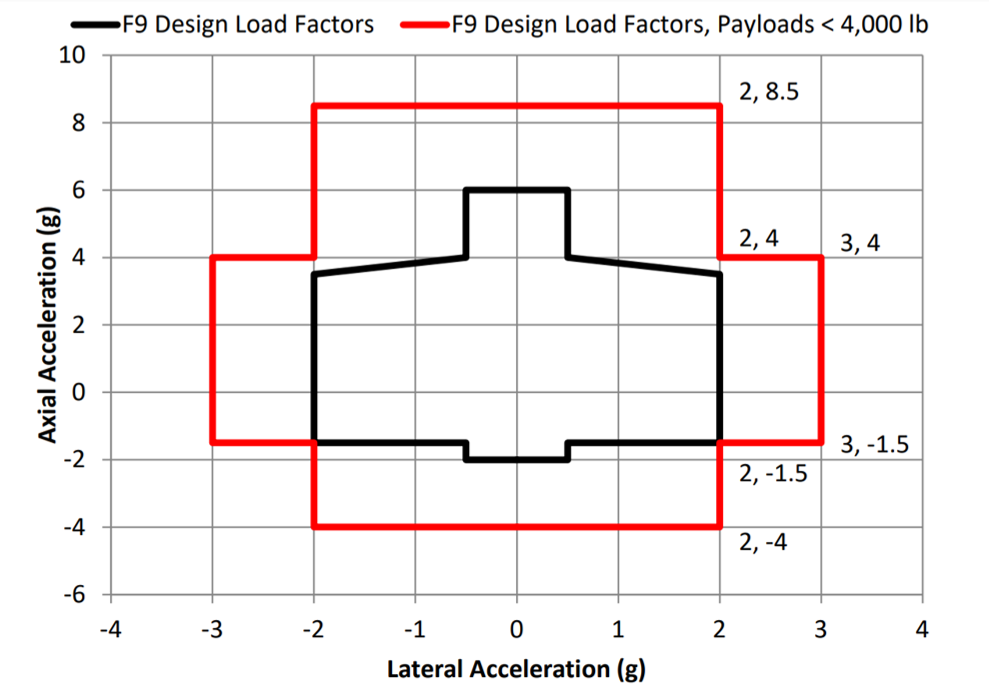
\includegraphics[width=\textwidth]{Img/falcon_static.png}
         \caption{Accélérations statiques axiales et latérales maximales}
         \label{fig:falcon9_static}
     \end{subfigure}
     \hfill
     \begin{subfigure}[]{0.48\textwidth}
         \centering
         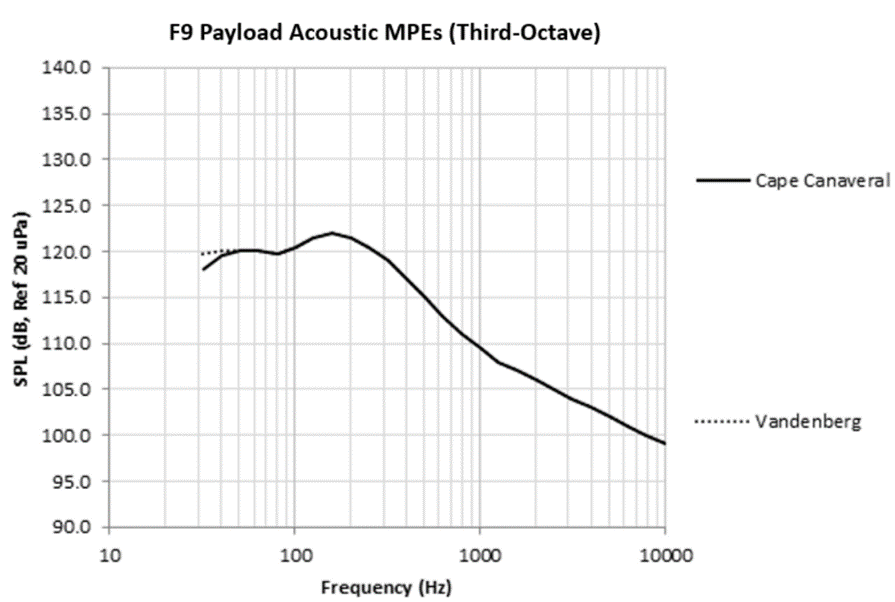
\includegraphics[width=\textwidth]{Img/falcon_acoustic.png}
         \caption{Environnement acoustique maximal prédit (P95/50)}
         \label{fig:falcon9_acoustic}
     \end{subfigure}
     \\
     \begin{subfigure}[]{0.48\textwidth}
         \centering
         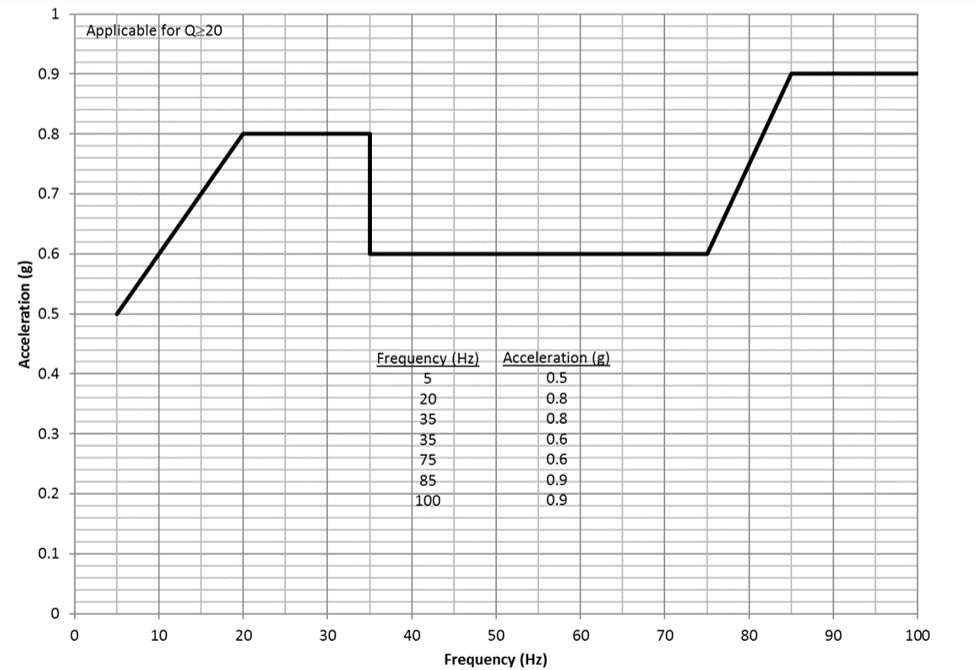
\includegraphics[width=\textwidth]{Img/falcon_sine.png}
         \caption{Environnement de vibration sinusoïdal maximal équivalent}
         \label{fig:falcon_sine}
     \end{subfigure}
     \hfill     
     \begin{subfigure}[]{0.48\textwidth}
         \centering
         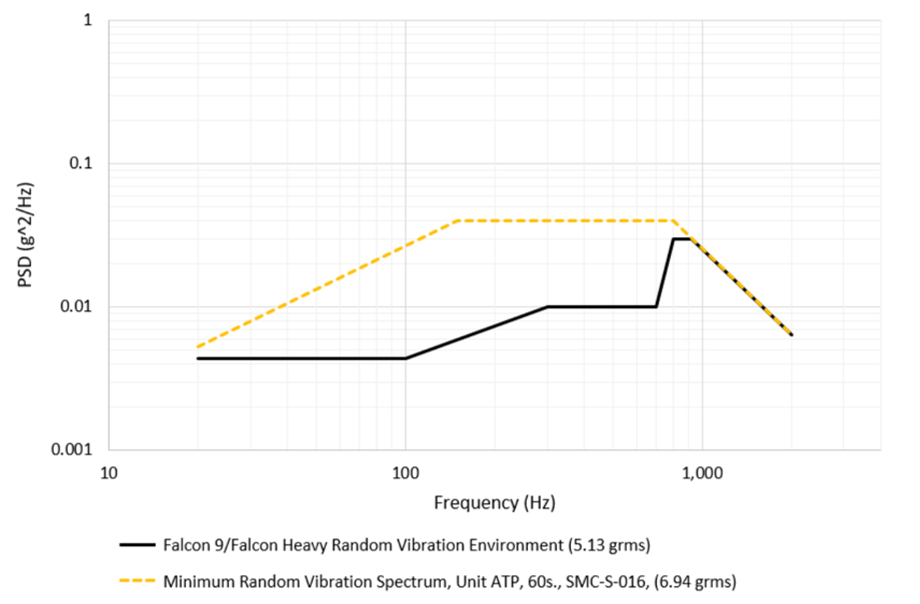
\includegraphics[width=\textwidth]{Img/falcon_random.png}
         \caption{Environnement de vibrations aléatoires maximum prédit (P95/50)}
         \label{fig:falcon_random}
     \end{subfigure}
     \caption{\centering{Charges maximales exercées sur le rover par l'environnement du lancement de la fusée Falcon 9. Tiré de \cite{SpaceExplorationTechnologiesCorp2020FalconGuide} } }.
     \label{fig:Falcon9}
\end{figure}

\setkeys{Gin}{draft=false} % Compile again figures

And now it compiles again 

\begin{figure}[h] %H impose the position after this text, h will place the figure as soon as possible
     \centering
     \begin{subfigure}[]{0.48\textwidth}
         \centering
         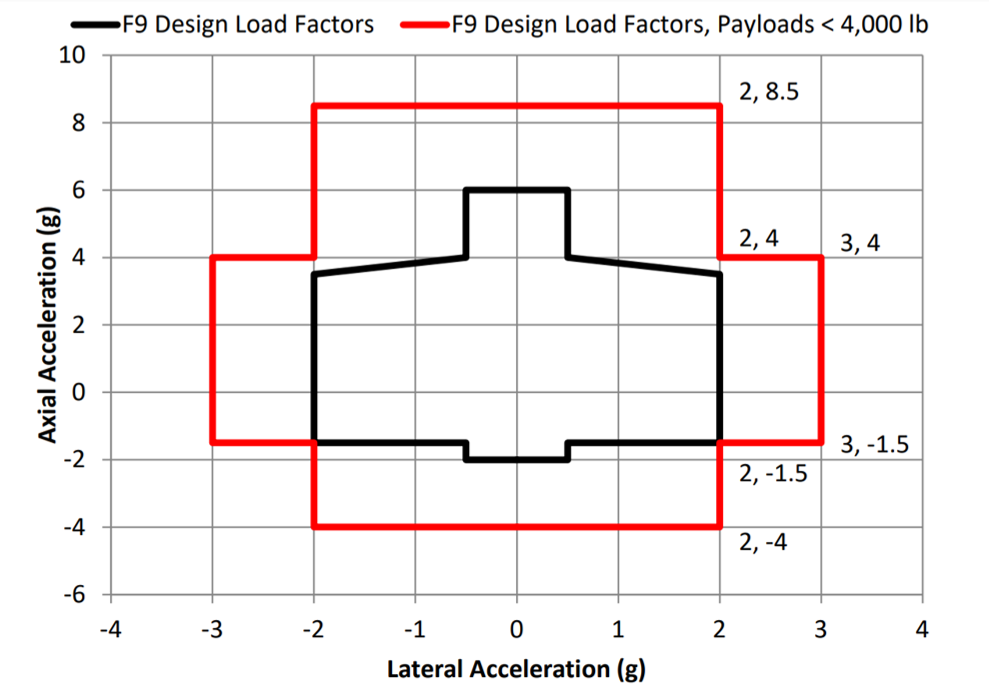
\includegraphics[width=\textwidth]{Img/falcon_static.png}
         \caption{Accélérations statiques axiales et latérales maximales}
         \label{fig:falcon9_static}
     \end{subfigure}
     \hfill
     \begin{subfigure}[]{0.48\textwidth}
         \centering
         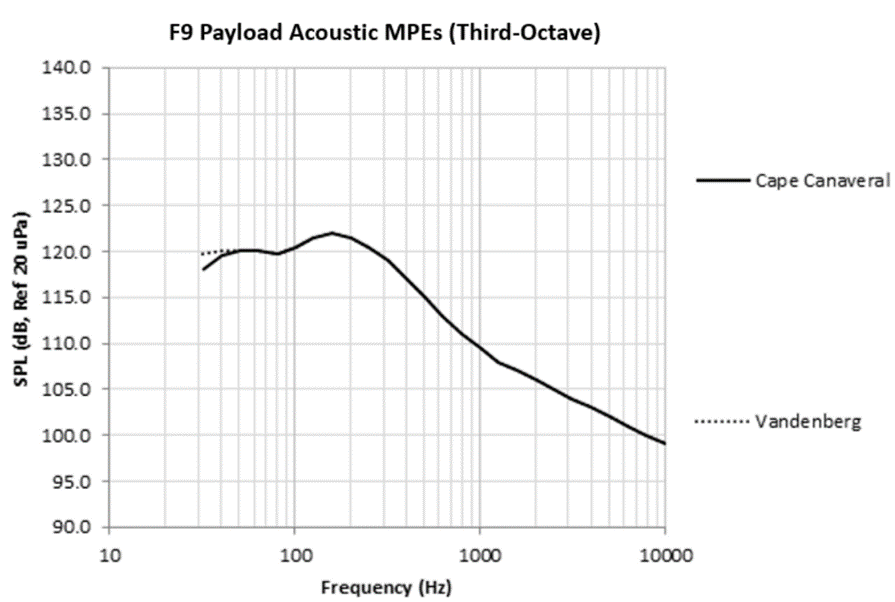
\includegraphics[width=\textwidth]{Img/falcon_acoustic.png}
         \caption{Environnement acoustique maximal prédit (P95/50)}
         \label{fig:falcon9_acoustic}
     \end{subfigure}
     \\
     \begin{subfigure}[]{0.48\textwidth}
         \centering
         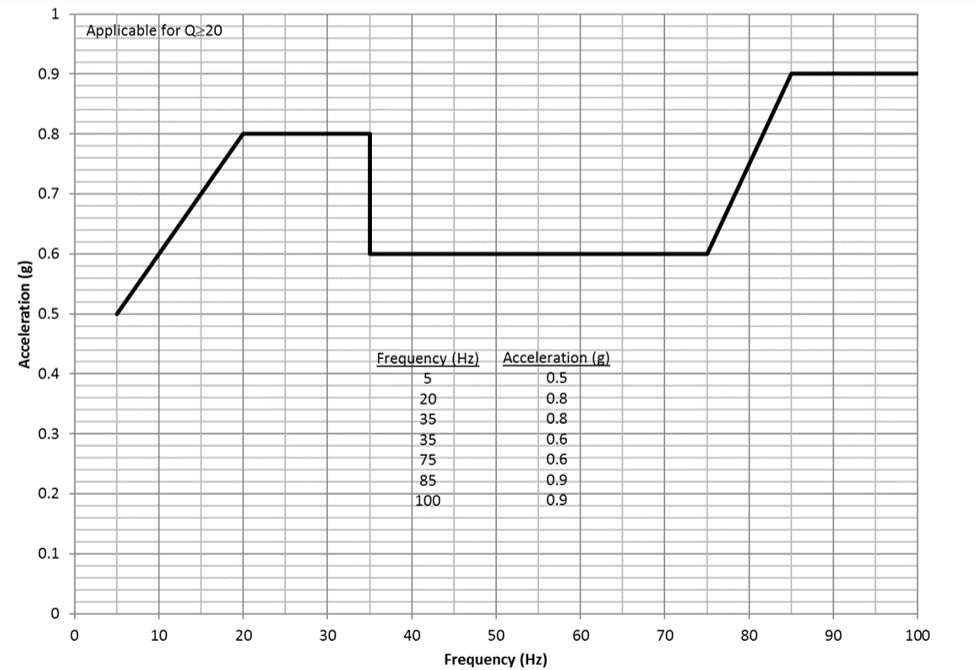
\includegraphics[width=\textwidth]{Img/falcon_sine.png}
         \caption{Environnement de vibration sinusoïdal maximal équivalent}
         \label{fig:falcon_sine}
     \end{subfigure}
     \hfill     
     \begin{subfigure}[]{0.48\textwidth}
         \centering
         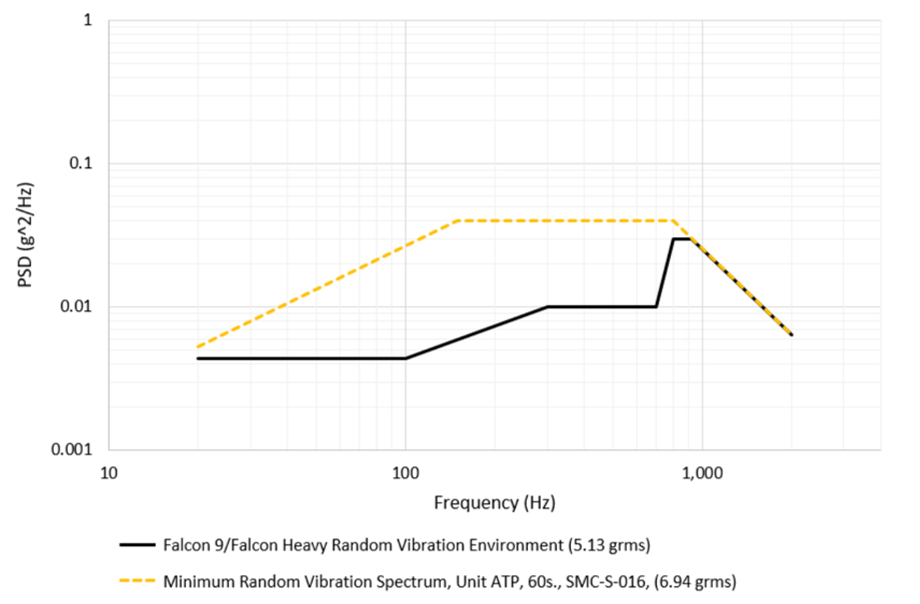
\includegraphics[width=\textwidth]{Img/falcon_random.png}
         \caption{Environnement de vibrations aléatoires maximum prédit (P95/50)}
         \label{fig:falcon_random}
     \end{subfigure}
     \caption{\centering{Charges maximales exercées sur le rover par l'environnement du lancement de la fusée Falcon 9. Tiré de \cite{SpaceExplorationTechnologiesCorp2020FalconGuide} } }.
     \label{fig:Falcon9}
\end{figure}